\chapter{Projection --- The Central Idea}
\label{ch:lesson30}

This begins Part 3: deep learning for computer vision, which focuses on the modern approaches that use neural networks. Before writing a single neural network, though, it's worth pausing to reflect upon an idea that rarely gets much attention despite its fundamental importance. \textbf{Projection} is a simple idea: map points from one space into another, usually a simpler one, by a linear combination of their coordinates. Projection quietly ran through much of Parts I and II --- many of the techniques so far have secretly been projections. Projection also underlies everything from here on: neural networks turn out to be nothing more than \emph{learned}, \emph{composed} projections.

\section{Two projections you've already built}

\textbf{PCA} (Chapter~\ref{ch:lesson06}). Given a cloud of points, the eigenvectors of their covariance matrix gave directions to project onto. Projecting onto the top eigenvector, $y=v^\top x$, collapses each 2D point to a single number --- the coordinate along the direction of greatest spread, as Figure~\ref{fig:l30-1} shows.

\begin{figure}[h]
\centering
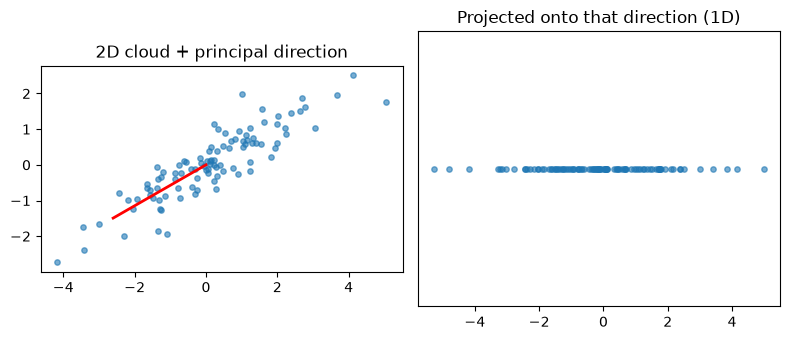
\includegraphics[width=0.75\textwidth]{figures/lesson30_fig01.png}
\caption{A 2D cloud with its principal direction, and the same points projected onto that direction (1D).}
\label{fig:l30-1}
\end{figure}

\textbf{Camera projection} (Chapters~\ref{ch:lesson24}--\ref{ch:lesson25}). $P=K[R|t]$ maps a 3D world point to a 2D pixel. Every row of that matrix, before the final homogeneous divide, is itself a linear projection: a dot product between the point's coordinates and a fixed direction, plus an offset.

Both examples share the same mechanics: pick a direction $w$ (and maybe an offset $b$), then compute $y=w^\top x+b$. What differs is \emph{why} the direction was chosen: PCA picks $w$ to maximize the spread of the projected data (an unsupervised, purely geometric objective); a camera's rows are fixed by its physical geometry. Neither is chosen to solve a classification or recognition problem --- but nothing stops us from choosing $w$ for exactly that purpose.

\section{Matrix multiplication: many projections at once}

Everything above computed one number $y=w^\top x$ from one direction $w$. Stack $m$ different directions as the rows of a matrix $W$ (shape $m\times n$), and $y=Wx$ computes all $m$ projections at once --- one dot product per row. This is exactly what matrix multiplication \emph{is}: a bank of simultaneous projections. Several seemingly different linear operations from earlier in this course are secretly the same operation, just with a different, structured choice of $W$:
\begin{itemize}
  \item \textbf{Convolution} (Chapter~\ref{ch:lesson10}): each output value is a dot product between a small neighborhood and a kernel --- a projection. Sliding the kernel across the whole signal is a matrix multiply by a sparse matrix whose rows are shifted copies of the kernel (a Toeplitz matrix).
  \item \textbf{The Fourier transform} (Chapter~\ref{ch:lesson15}): each output value is a dot product between the \emph{whole} signal and one sinusoid at a fixed frequency --- a projection onto that frequency. The full transform is a matrix multiply by a fixed matrix of sines and cosines.
  \item \textbf{A homography or camera projection matrix} (Chapters~\ref{ch:lesson24}--\ref{ch:lesson25}): each output coordinate is a dot product between a homogeneous point and one row of $H$ or $P$.
\end{itemize}
Verified directly: a hand-built Toeplitz matrix reproduces \code{np.convolve} to within $5.6\times10^{-17}$, and a hand-built matrix of sinusoids reproduces \code{np.fft.fft} to within $2.9\times10^{-15}$ --- both effectively exact, floating-point roundoff only.

A fully-connected neural network layer is nothing more than this same $y=Wx+b$, with $W$'s rows \emph{learned} to solve a task instead of fixed by hand-derived structure (a kernel shape, a bank of sinusoids, a camera's geometry).

\section{A projection for classification}

Suppose instead of ``maximize spread,'' the goal is ``separate two classes.'' The same formula $y=w^\top x+b$ still applies --- project each point onto a direction $w$, and classify by the \emph{sign} of the resulting score. This is, in its entirety, a single artificial neuron with no activation function: the linear core that every neural network layer is built from.

A principled hand-picked direction --- pointing from one class's mean toward the other's, with the threshold at the midpoint --- reaches $100.0\%$ classification accuracy on two well-separated synthetic classes (Figure~\ref{fig:l30-2}).

\begin{figure}[h]
\centering
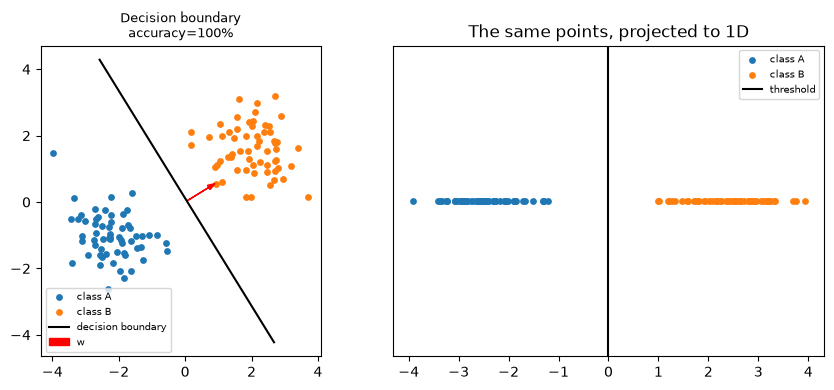
\includegraphics[width=0.9\textwidth]{figures/lesson30_fig02.png}
\caption{Left: the decision boundary in the original 2D space, perpendicular to $w$. Right: the same points projected down onto $w$, with classification reduced to thresholding a single number at zero. The 2D picture is more intuitive, but the 1D picture is what actually generalizes --- in 100 dimensions there's no picture to draw of the ``boundary,'' but ``project to a single number, then threshold'' still works exactly the same way.}
\label{fig:l30-2}
\end{figure}

\section{What a single projection cannot do}

A single linear projection can only produce a \emph{straight-line} decision boundary (a hyperplane, in higher dimensions). Some datasets have no straight-line separator at all --- the classic example is one class surrounding the other. Searching 2000 random directions and 61 thresholds each for the best possible linear separator between a ring and a surrounded disk finds a best achievable accuracy of just $74.2\%$, as Figure~\ref{fig:l30-3} shows.

\begin{figure}[h]
\centering
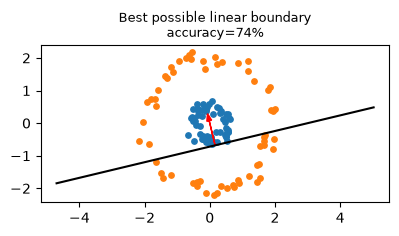
\includegraphics[width=0.45\textwidth]{figures/lesson30_fig03.png}
\caption{The best possible linear boundary between a disk and a surrounding ring --- no rotation or shift of a single straight line can separate them, so the best any linear projection can manage is a mediocre compromise.}
\label{fig:l30-3}
\end{figure}

This is the wall every purely linear method runs into, and it's exactly what motivates the next two chapters: first, \emph{learning} $w$ and $b$ automatically instead of hand-picking them, and then, more importantly, \emph{composing several projections with nonlinearities in between}, which, given enough capacity, can separate regions of essentially any shape.

\subsection*{Exercises}
\begin{enumerate}
  \item In the PCA recap, project the cloud onto the \emph{second} (smaller) eigenvector instead of the principal one. How does the spread of the resulting 1D projection compare to projecting onto the principal direction, and why does that match what the eigenvalue itself tells you (Chapter~\ref{ch:lesson06})?
  \item Modify the two classes' means and spread so they overlap more. At what point does the mean-difference direction $w$ stop achieving high accuracy, and can you find a \emph{better} $w$ than the mean-difference one by hand for that harder case?
  \item For the ring-and-disk dataset, instead of a linear projection, try classifying by a simple nonlinear function of the points: the distance from the origin, $r=\sqrt{x_1^2+x_2^2}$, thresholded at some value. What accuracy does this one nonlinear feature achieve, and what does that suggest about \emph{what kind} of projection would actually solve this problem?
\end{enumerate}

\vfill
\fullcode{lesson30}{lesson30_projection}
